\documentclass[tikz,border=8pt]{standalone}
\usetikzlibrary{arrows.meta,calc,decorations.pathmorphing}

\begin{document}
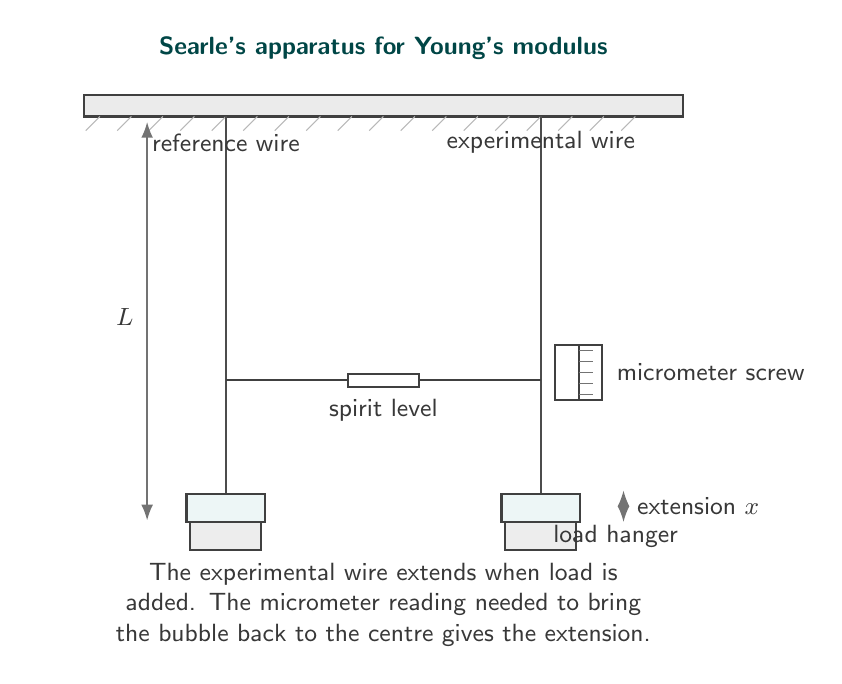
\begin{tikzpicture}[
  line/.style={draw=black!75,line width=0.75pt},
  wire/.style={draw=black!70,line width=0.55pt},
  label/.style={font=\sffamily\small,text=black!78},
  title/.style={font=\sffamily\bfseries\small,text=teal!55!black},
  dim/.style={{Latex[length=2mm]}-{Latex[length=2mm]},draw=black!55,line width=0.55pt},
]

\node[title] at (0,4.42) {Searle's apparatus for Young's modulus};
\draw[line,fill=black!8] (-3.8,3.55) rectangle (3.8,3.82);
\foreach \x in {-3.6,-3.2,...,3.6}
  \draw[black!28] (\x,3.55) -- ++(-0.18,-0.18);

\draw[wire] (-2.0,3.55) -- (-2.0,-1.6);
\draw[wire] (2.0,3.55) -- (2.0,-1.6);
\node[label] at (-2.0,3.22) {reference wire};
\node[label] at (2.0,3.22) {experimental wire};

\draw[line,fill=teal!7] (-2.5,-1.6) rectangle (-1.5,-1.25);
\draw[line,fill=teal!7] (1.5,-1.6) rectangle (2.5,-1.25);
\draw[line,fill=black!7] (-2.45,-1.95) rectangle (-1.55,-1.6);
\draw[line,fill=black!7] (1.55,-1.95) rectangle (2.45,-1.6);
\node[label] at (2.95,-1.78) {load hanger};

\draw[line,fill=white] (-2.0,0.2) -- (2.0,0.2);
\draw[line,fill=white] (-0.45,0.12) rectangle (0.45,0.28);
\node[label,below] at (0,0.08) {spirit level};
\draw[line,fill=white] (2.18,-0.05) rectangle (2.78,0.65);
\draw[line] (2.48,-0.05) -- (2.48,0.65);
\foreach \y in {0.02,0.16,0.30,0.44,0.58}
  \draw[black!55] (2.48,\y) -- ++(0.18,0);
\node[label,right] at (2.84,0.3) {micrometer screw};

\draw[dim] (-3.0,3.48) -- (-3.0,-1.58);
\node[label,left] at (-3.05,1.0) {$L$};
\draw[dim] (3.05,-1.6) -- (3.05,-1.2);
\node[label,right] at (3.1,-1.4) {extension $x$};

\node[label,align=center,text width=8.8cm] at (0,-2.65)
  {The experimental wire extends when load is added. The micrometer reading needed to bring the bubble back to the centre gives the extension.};

\end{tikzpicture}
\end{document}
